\documentclass[12pt]{article}

\usepackage{graphicx}   % need for figures

% don't need the following. simply use defaults
\setlength{\baselineskip}{16.0pt}    % 16 pt usual spacing between lines

\setlength{\parskip}{3pt plus 2pt}
\setlength{\parindent}{20pt}
\setlength{\oddsidemargin}{0.5cm}
\setlength{\evensidemargin}{0.5cm}
\setlength{\marginparsep}{0.75cm}
\setlength{\marginparwidth}{2.5cm}
\setlength{\marginparpush}{1.0cm}
\setlength{\textwidth}{150mm}

\graphicspath{{../figures/}}


% above is the preamble

\begin{document}

\title{Assignment 5}
\author{William Richard}
\maketitle

\section{Accuracies and Standard Deviations}

\begin{table}[ht]
\begin{tabular}{l || p{2cm} | p{2cm} | p{2cm} |  p{2cm}}
algorithm& A& B& C& ionosphere\\
\hline
\hline
generativeSharedCov & 0.952 +/- 0.0175& 0.850 +/- 0.0548& 0.830 +/- 0.0458& 0.855 +/- 0.0592\\
\hline
generativeSeperateCov& 0.515 +/- 0.0376& 0.550 +/- 0.1225& 0.515 +/- 0.1566& 0.641 +/- 0.0697\\
\hline
fishersLinearDiscriminent& 0.054 +/- 0.0138& 0.150 +/- 0.0806& 0.160 +/- 0.0663& 0.128 +/- 0.0514\\
\hline
logisticRegression& 0.485 +/- 0.038& 0.645 +/- 0.111& 0.700 +/- 0.114& 0.661 +/- 0.076\\ 
\end{tabular}
\label{tab:accStdDev}
\caption{Mean accuracy +/- 1 standard deviation for all algorithms on all datasets}
\end{table}

Surprisingly, the generative model with shared covariance matrices did best in all cases, not only with the highest average accuracy but also the lowest standard deviations.  

\section{Learning Curves}

With all algorithsm on all datasets, the training size does not seem to have a profound effect.  It does help to have larger training sets, but in most cases the training set size did not drastically effect the preformance of the algorithm.

Interestingly, on dataset A, having a training set of size 1000 with the generative regression with seperate covariance matricies saw a great improvement in performance.  This is likely random chance, rather than meaningful improvement.  See fig \ref{fig:A}.

It is possible that I did not impliment logistic regression correctly - for some datasets, like B and C (see figures \ref{fig:B} and \ref{fig:C}) it looks like some variation occured for different sized training sets, while for the A and ionosphere datasest (figures \ref{fig:A} and \ref{fig:ionosphere}) no difference appeared to occur when training set changed.  Also, the logistic training  took a very long time - on the order of 8-10 minutes per fold on dataset A.

It appears that though the generative model  with shared covariances is one of the simlier algorithms that we explored, in almost all scenarios it performed best, with the highest mean accuracy and smallest standard deviations from that mean.

\begin{figure}[h]
\centering
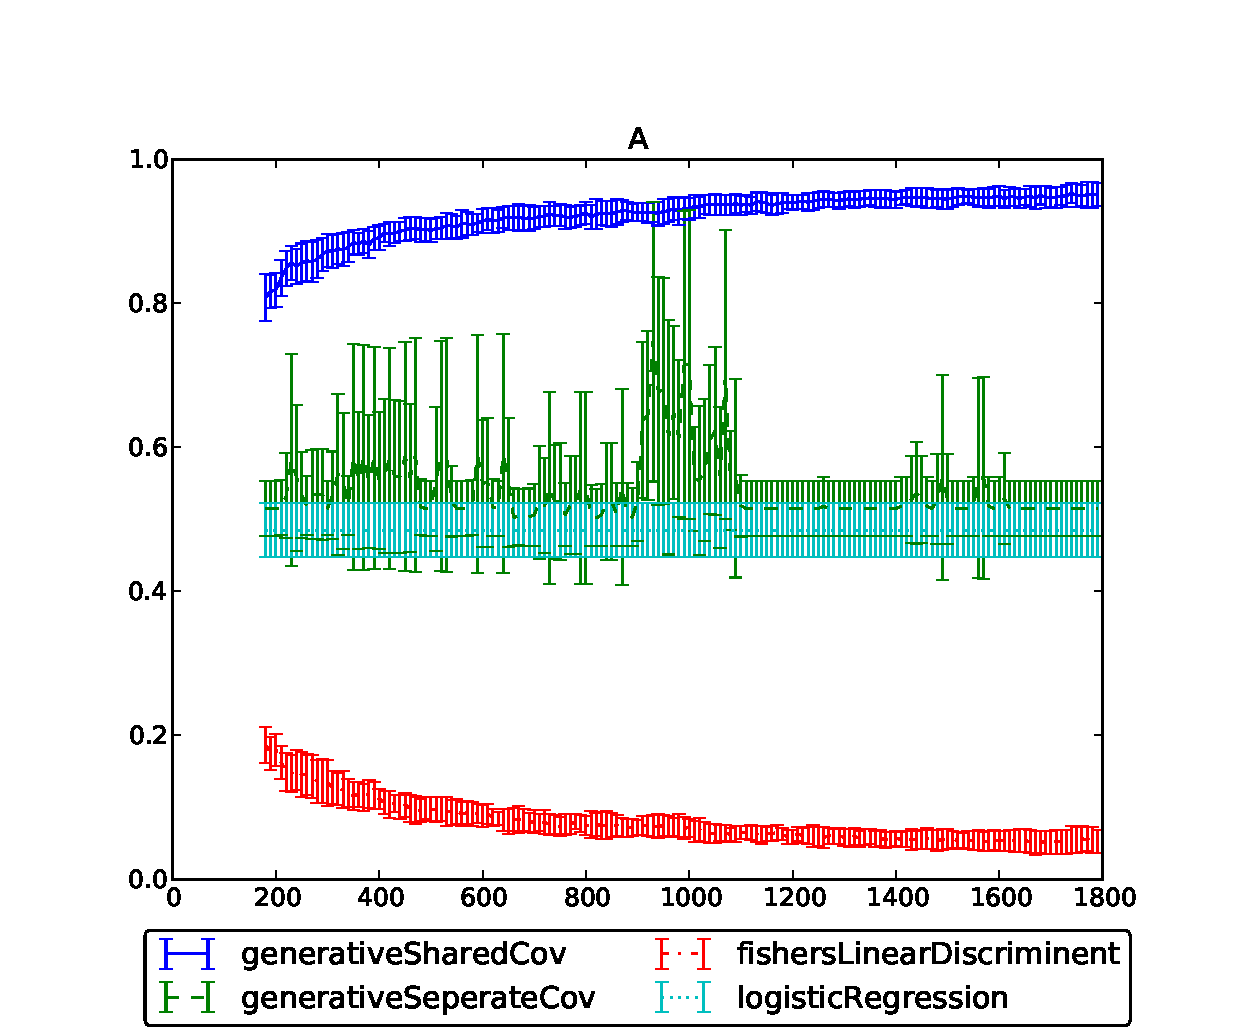
\includegraphics[width=.9\textwidth]{A-learning_curve.pdf};
\caption{Learning Curves on the A dataset}
\label{fig:A}
\end{figure}

\begin{figure}[h]
\centering
\vspace{-1.5in}
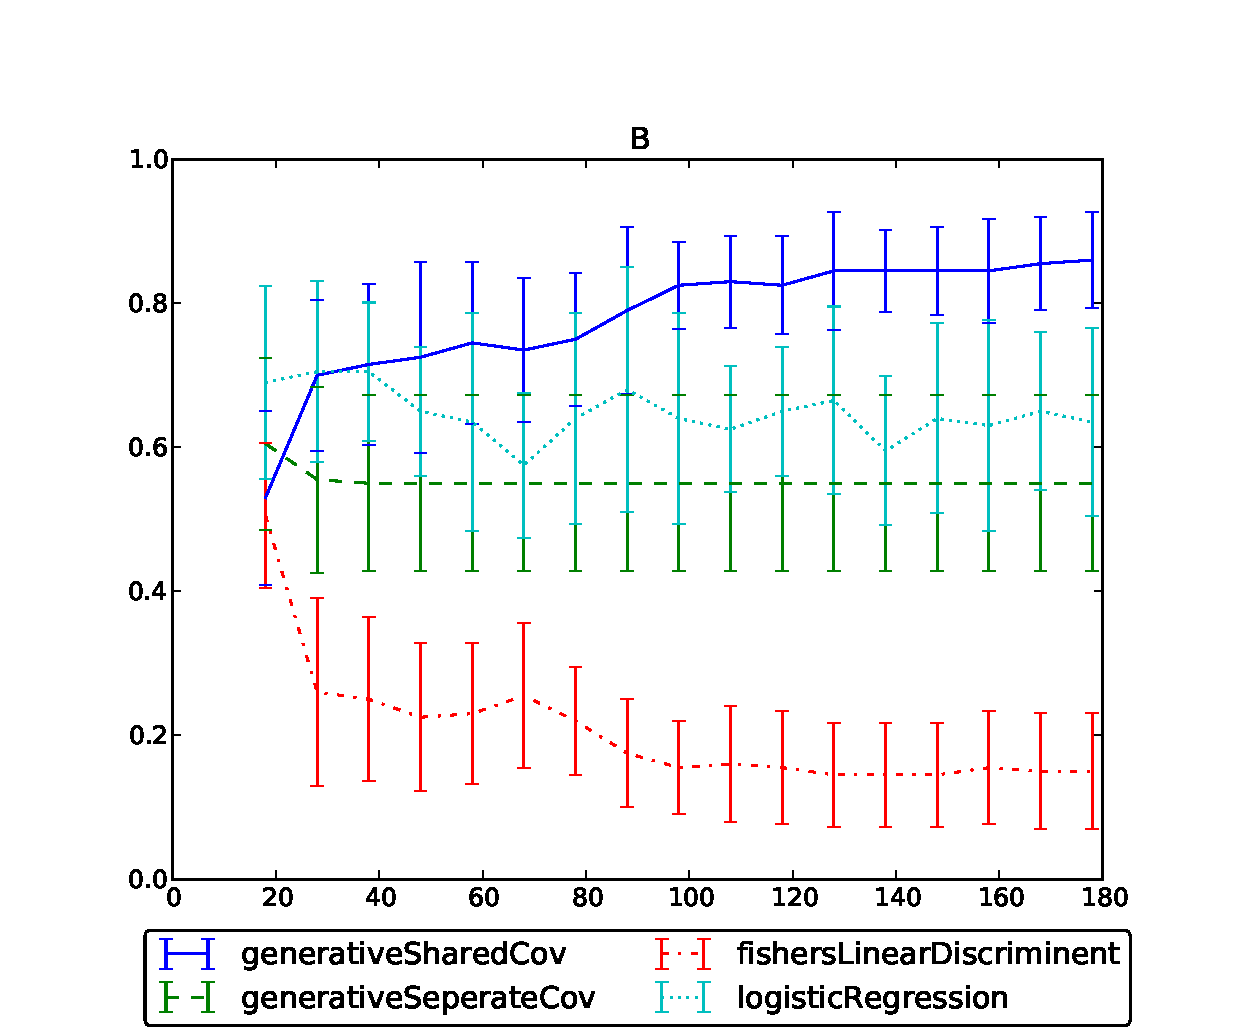
\includegraphics[width=.85\textwidth]{B-learning_curve.pdf}
\caption{Learning Curves on the B dataset}
\label{fig:B}
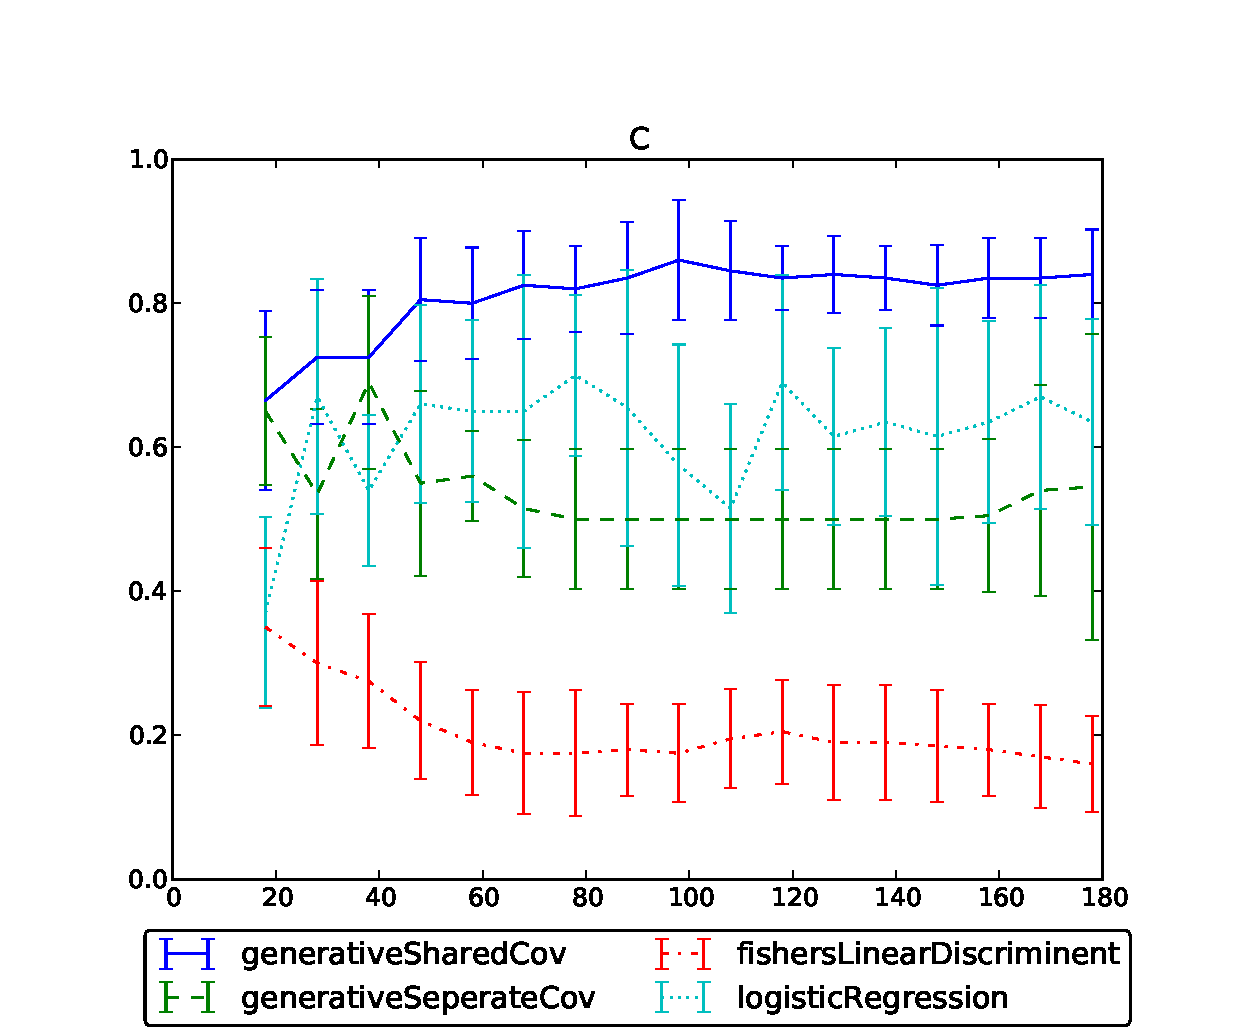
\includegraphics[width=.85\textwidth]{C-learning_curve.pdf}
\caption{Learning Curves on the C dataset}
\label{fig:C}
\end{figure}

\begin{figure}[h]
\centering
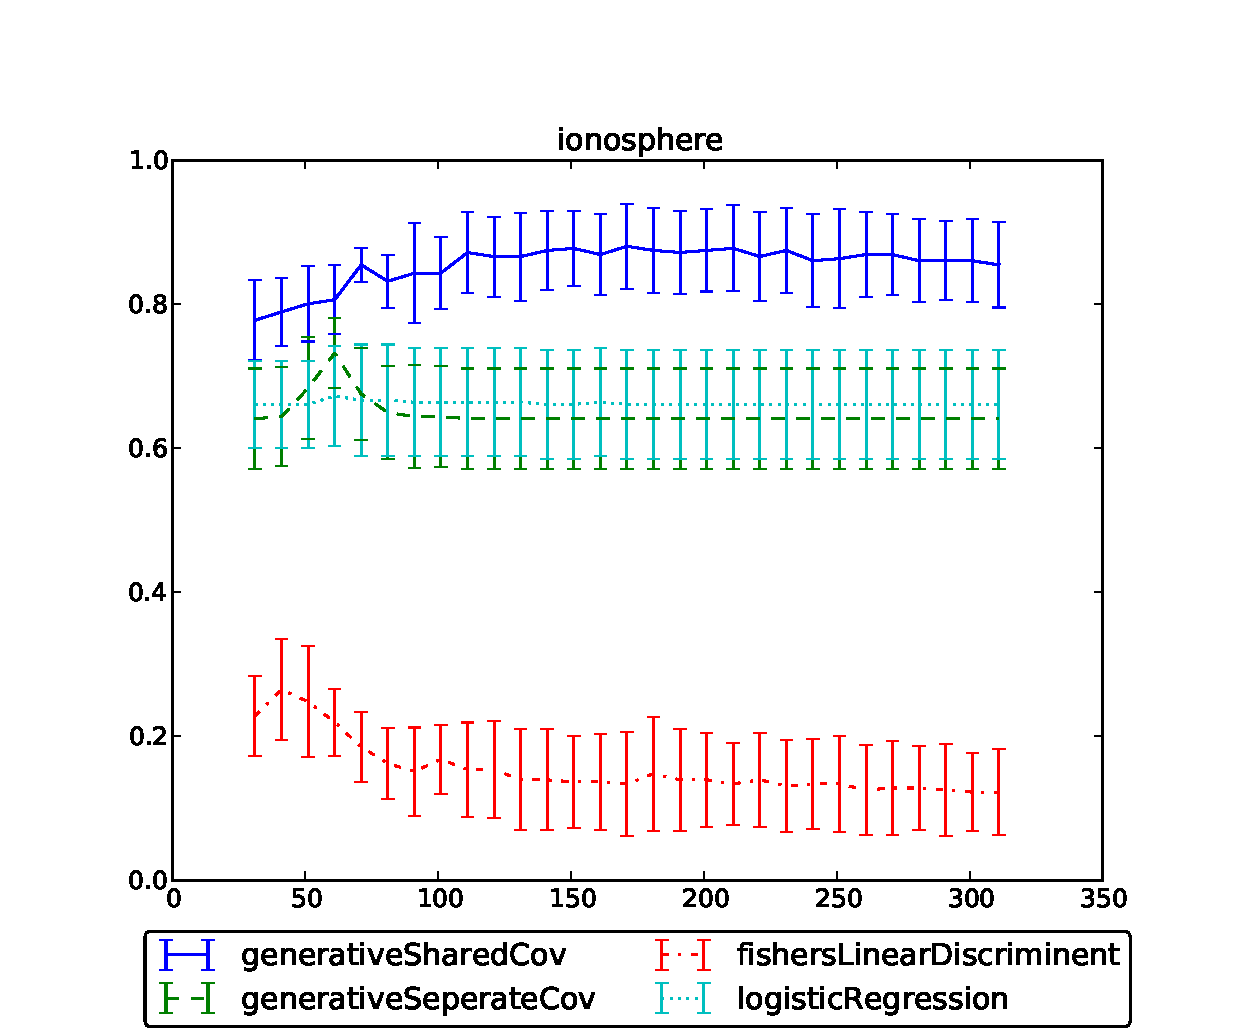
\includegraphics[width=\textwidth]{ionosphere-learning_curve.pdf}
\caption{Learning Curves on the ionosphere dataset}
\label{fig:ionosphere}
\end{figure}





\end{document}